\chapter{Desenvolvimento do novo Portal \\FlossCoach}
\label{desenvolvimento}

O desenvolvimento do novo Portal FlossCoach foi dividido em três fases. Na primeira, 
nós construimos um protótipo funcional com base no FlossCoach desenvolvido pelo professor 
Igor Steinmancher. Nós começamos o
desenvolvimento do protótipo funcional pelos motivos citados na Seção~\ref{flosscoach}.

O objetivo da primeira fase do desenvolvimento era que tivéssemos como cadastrar 
os projetos com os campos para cadastro que já eram relatados no portal FlossCoach 
além de um cadastro de usuários.

Para a obtenção desse cadastro, tivemos algumas conversas com o professor Igor Steinmancher
para que chegássemos a um modelo de dados inicial, onde contivesse todos os itens que 
já estavam presentes no FlossCoach atual e os relacionamentos que ele gostaria que 
houvessem entre os elementos.

\begin{figure}[h]
	\centering
	\label{fig:diagrama_iicial}
		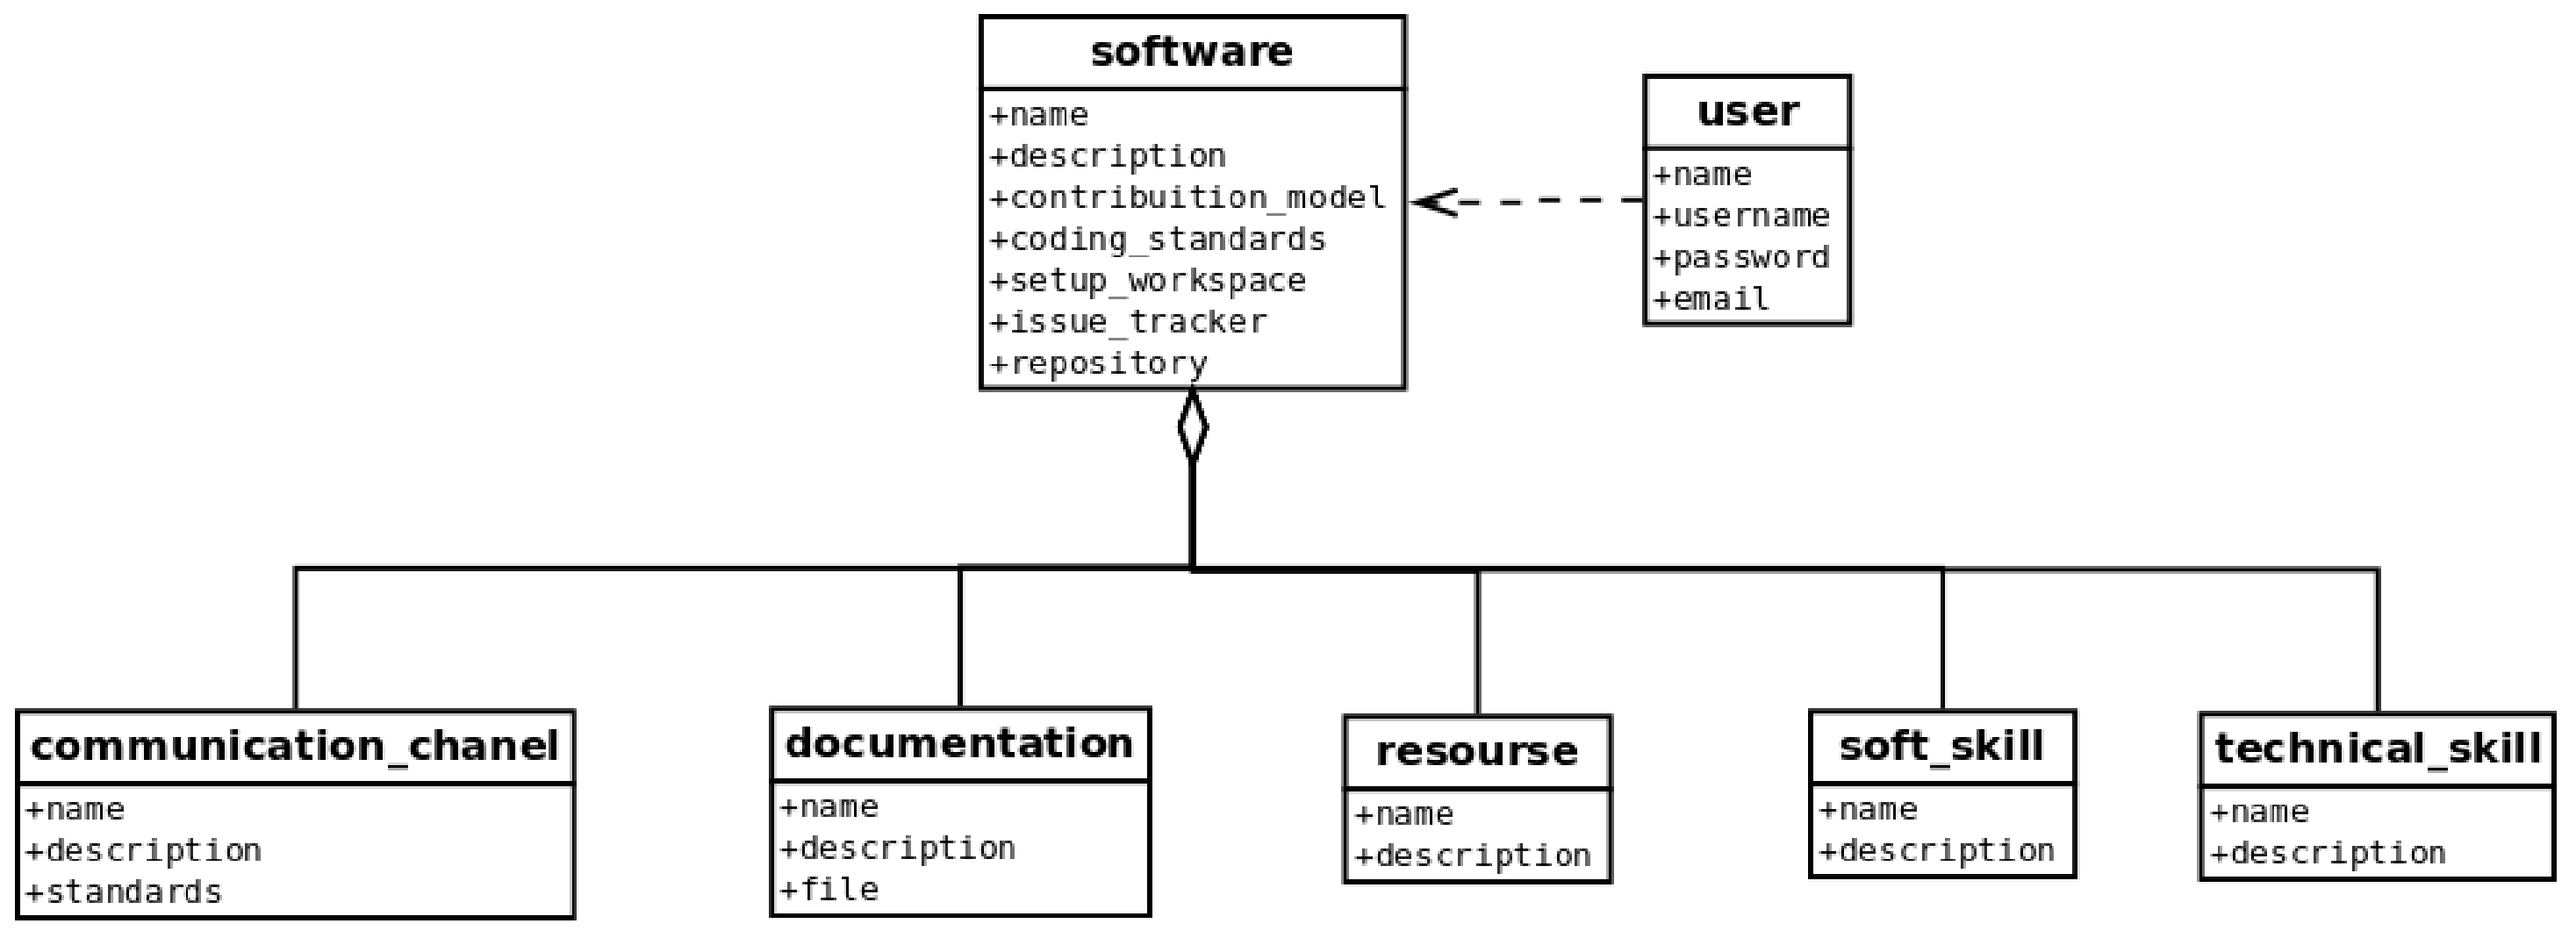
\includegraphics[keepaspectratio=true,scale=0.35]{figuras/diagrama_inicial.eps}
	\caption{Modelo de dados inicial do novo FlossCoach.}
\end{figure}

O protótipo funcional foi desenvolvido em \textit{ruby on rails} e \textit{bootstrap},
nós escolhemos estas tecnologias por serem amplamente utilizadas para desenvolvimento
de aplicações \textit{web} pela comunidade de software livre. Procuramos também utilizar
apenas recursos de software livre para o desenvolvimento, incluindo a ferramenta de 
controle de versão e as bibliotecas utilizadas no \textit{front end}. O código da classe
software, principal classe do projeto, pode ser visto no Apêndice~\ref{apendice1}.

Esta fase do desenvolvimento durou 4 meses, iniciamos levantando os dados para implementação
em dezembro de 2015 e concluimos em março de 2016 quando nós passamos a interagir de fato com o
professor Igor Steinmancher iniciando a segunda fase do desenvolvimento.  

\begin{figure}[h]
	\centering
	\label{fig:prototipo}
		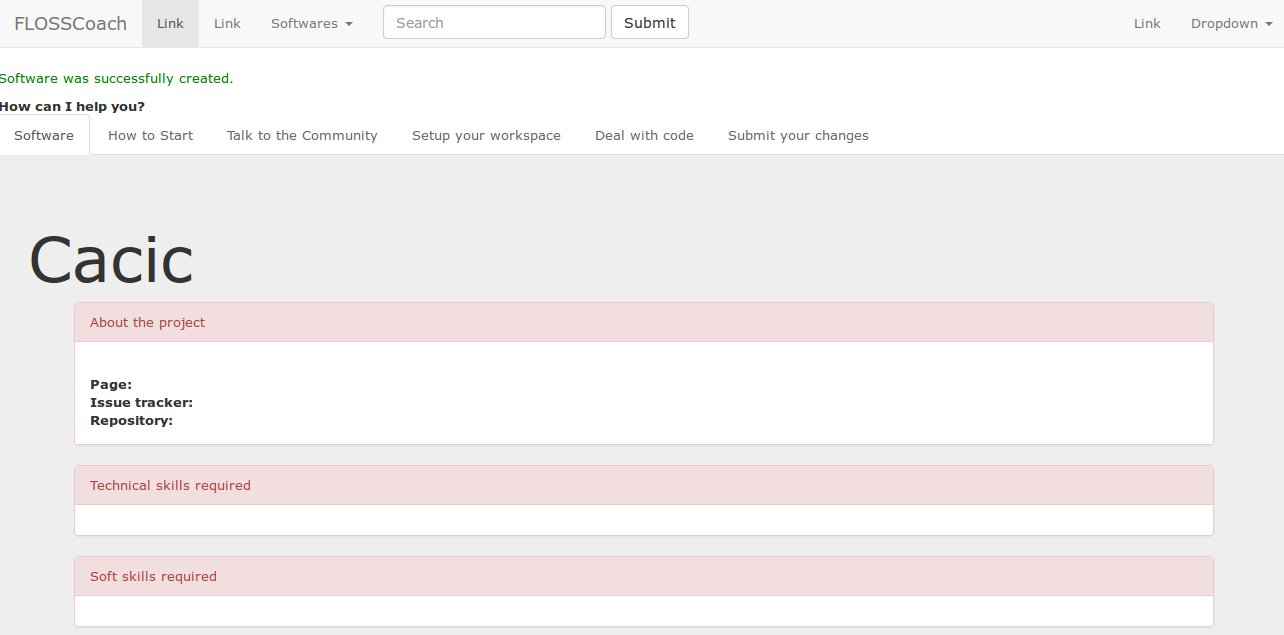
\includegraphics[keepaspectratio=true,scale=0.3]{figuras/prototipo.eps}
	\caption{Protótipo inicial do novo FlossCoach.}
\end{figure}

Na segunda fase do desenvolvimento o professor Igor Steinmancher montou uma equipe 
de bolsistas para o desenvolvimento, eles iniciaram uma análise do que nós havímos desenvolvido
e fizeram modificações no modelo de dados da aplicação chegando a uma segunda versão do 
modelo.

\begin{figure}[h]
	\centering
	\label{fig:diagrama_fase2}
		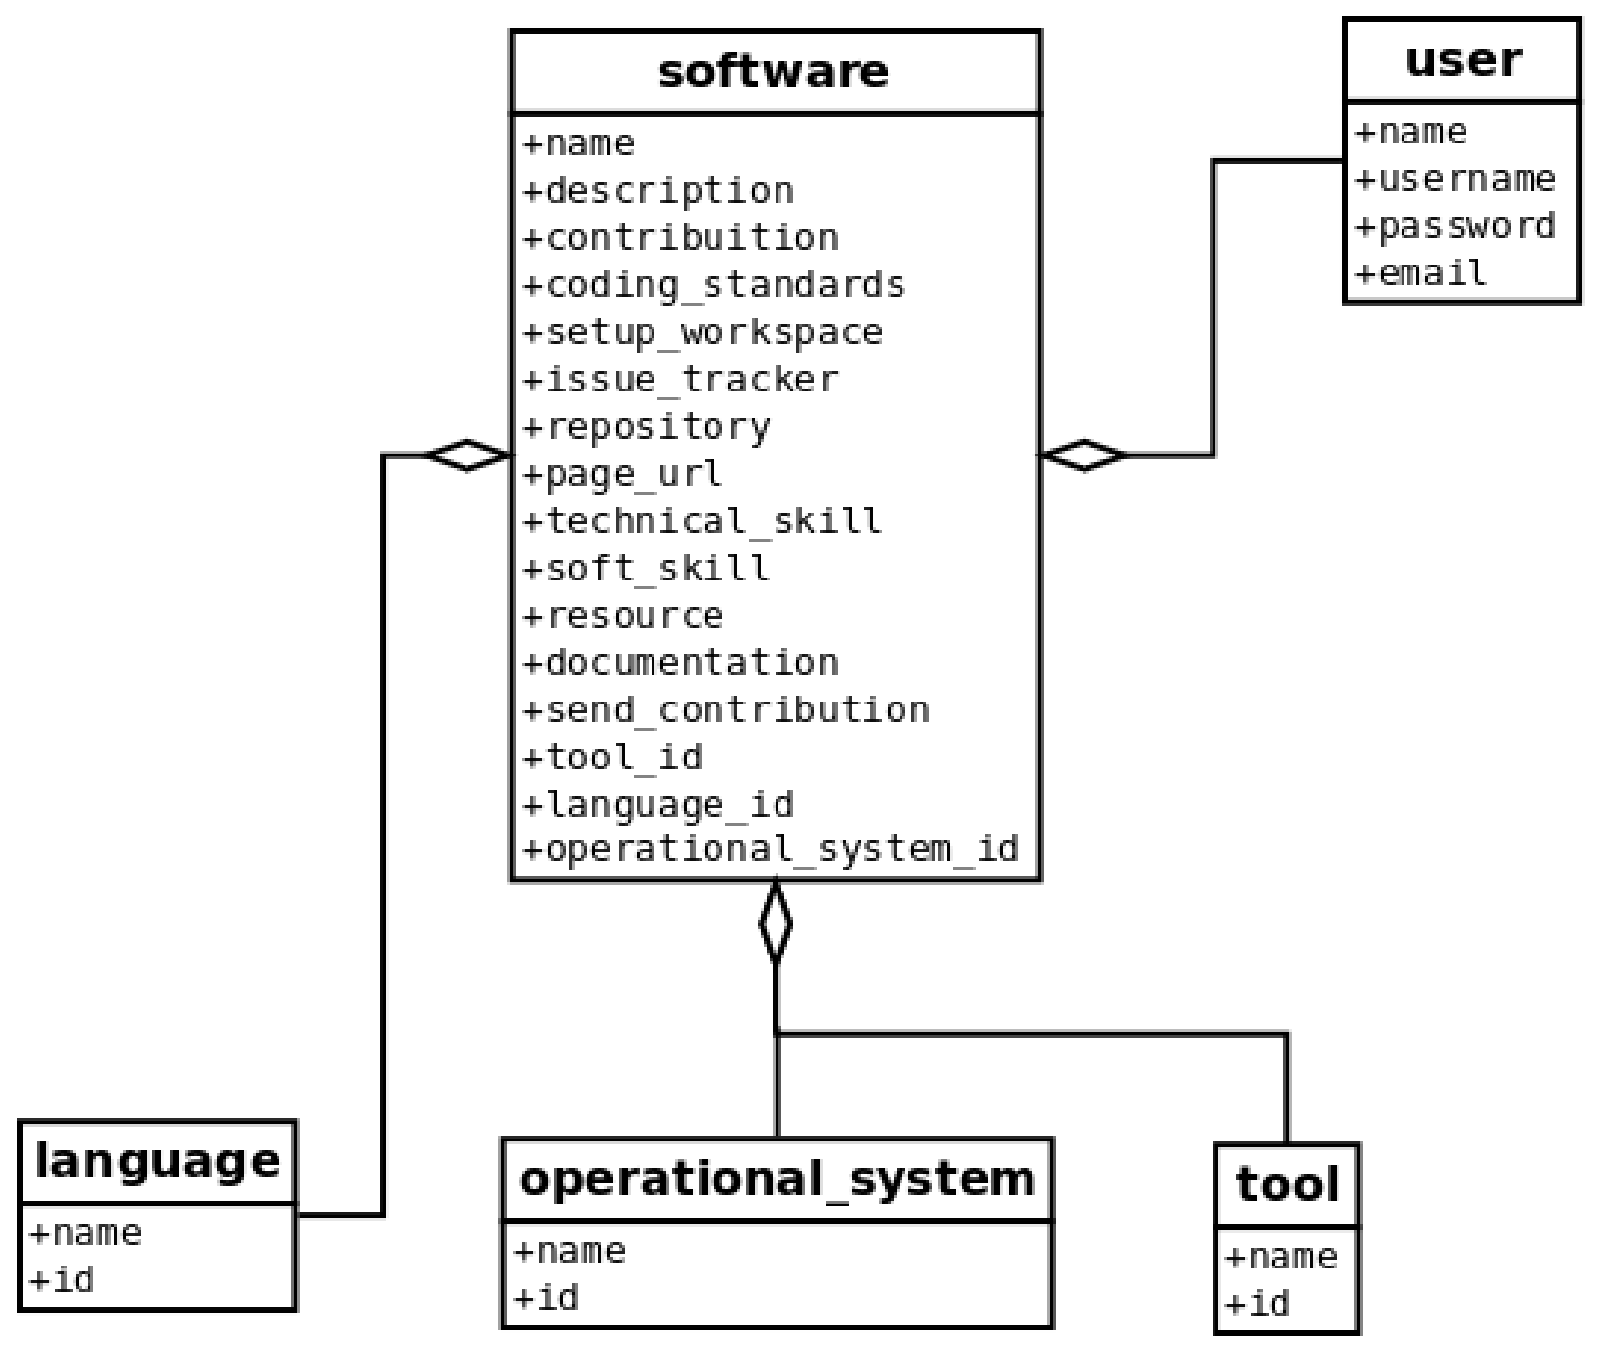
\includegraphics[keepaspectratio=true,scale=0.3]{figuras/diagrama_fase2.eps}
	\caption{Segunda versão do modelo de dados do novo FlossCoach.}
\end{figure}

Nessa segunda versão do modelo de dados algumas entidades deixaram de exixtir e se tornaram
atributos da classe \textit{software} e eles apresentaram 3 novas classes que não havia
no diagrama anterior. Eles implemetaram as modificações que fizeram no diagrama de dados
e melhoraram o \textit{front end} da aplicação além de desenvolver novas funcionalidades. 
Nesta etapa eles desenvolveram:
\begin{itemize}
\item Novo \textit{design} da aplicação;
\item Página de \textit{login}; 
\item \textit{Login} através de redes sociais;
\item Menu com barra lateral;
\item Modo tela cheia.
\item Consumo da API do \textit{Open hub}.
\end{itemize}

\begin{figure}[h]
	\centering
	\label{fig:prototipo}
		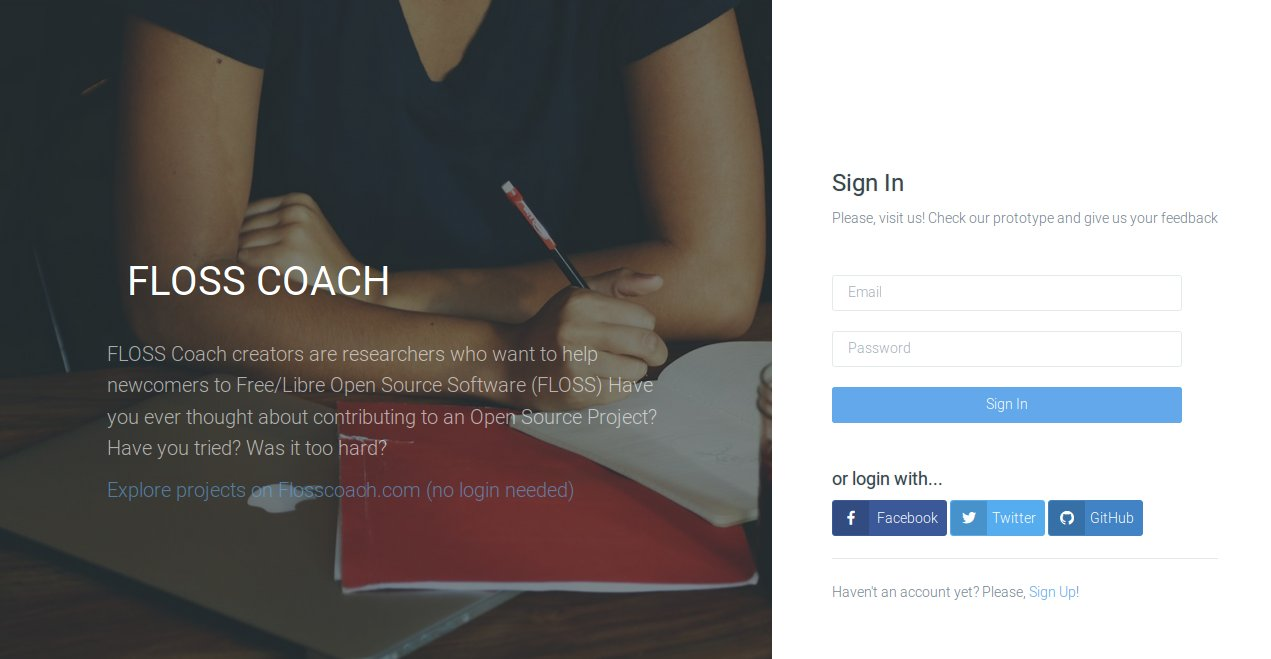
\includegraphics[keepaspectratio=true,scale=0.3]{figuras/login.eps}
	\caption{Página de \textit{login} inicial do novo FlossCoach.}
\end{figure}


\begin{figure}[h]
	\centering
	\label{fig:prototipo}
		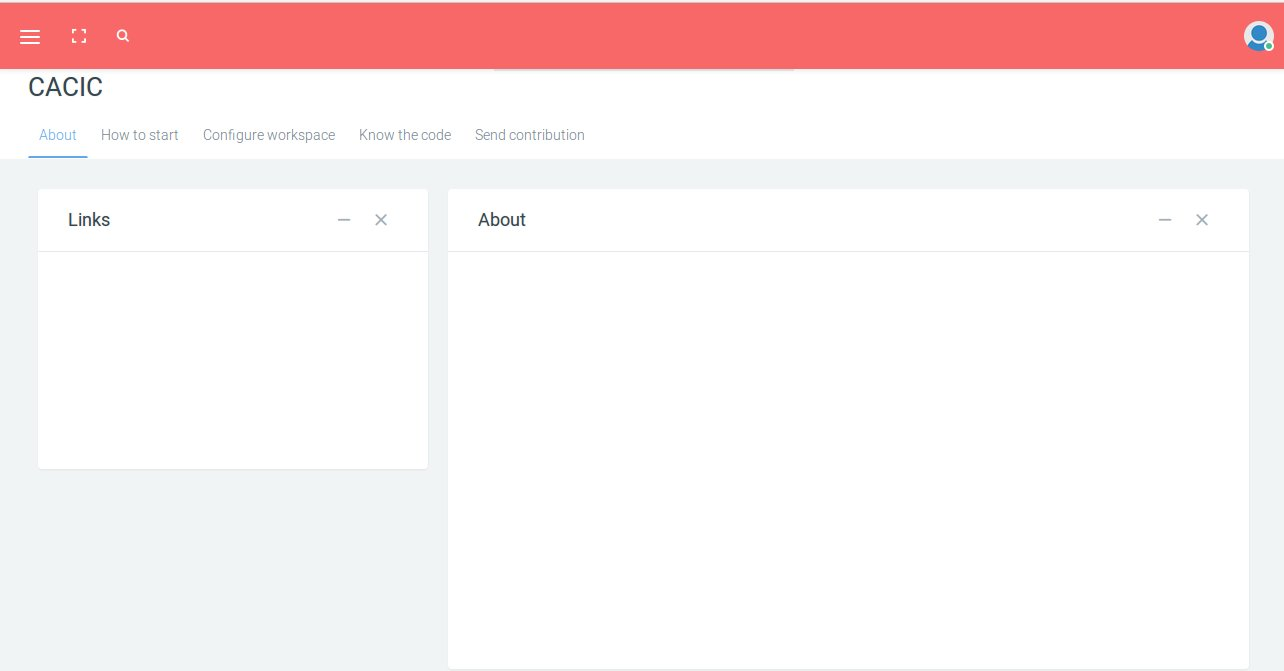
\includegraphics[keepaspectratio=true,scale=0.3]{figuras/layout.eps}
	\caption{\textit{Layout} do novo FlossCoach.}
\end{figure}


Nesse intervalo de tempo da segunda fase, nós trabalhamos na pesquisa das barreiras para
contribuir com software público. Esta fase também durou 4 meses, tendo início em abril 
de 2016 e finalizando em julho de 2016.

Iniciamos a terceira fase do desenvolvimento em agosto de 2016 juntamente com a disciplina 
de manutenção e evolução de software, minitrada pelo professor Paulo Meirelles na UnB. 
Nesta disciplina os alunos escolhem um projeto que queiram participar entre algumas opções 
e uma dessas opções foi o FlossCoach. O FlossCoach foi um dos 
projetos mais escolhidos pelos alunos e o professor Paulo Meirelles fez uma seleção
dos alunos para o desenvolvimento. Após essa seleção foi montada uma equipe com
6 alunos para desenvolver o projeto.

Essa disciplina tem como objetivo aplicar técnicas de desenvolvimento colaborativo,
são utilizados apenas projetos de software livre na disciplina para que os alunos 
possam se apropriar do código e assim fazer manutenções corretivas e evolutivas no
mesmo.

\begin{table}[h]
	\centering
	\begin{tabular}{ccc}
		\toprule
		\textbf{Sprint} & \textbf{Issues desenvolvidas} \\
		\midrule
		Sprint 1 & Levantar ambiente e tomar conhecimento do FlossCoach \\
			 & Configurar ambiente de testes unitários \\
			 & Escrita de testes de unidade das classes de modelos\\
		\midrule
		Sprint 2 & Criar papel de administrador do projeto\\
			 & Atribuir papel de administrador ao usuário que cria o projeto \\
			 & Aprovação de membros em projetos \\
		\midrule		
		Sprint 3 & Configuração da internacionalização \\
			 & Adicionar novos campos ao cadastro de usuário\\
			 & Redirecionar o \textit{link} de perfil para a página de perfil do usuário.\\
			 & Testes de papel de administrador.\\
		\midrule		
		Sprint 4 & Traduzir \textit{homepage}.\\
			 & Traduzir página de projetos.\\
			 & Traduzir página de perfil de usuário\\
			 & Traduzir cadastro de usuário.\\ 
			 & Permitir usuários a editar o seu perfil\\
			 & Corrigir erro de cadastro de e-mail já registrado.\\
			 & Estudar uma \textit{gem} de sistema de \textit{loging}.\\  
		\midrule		
		Sprint 5 & Implementar práticas de código limpo.\\
			 & Refatoração de código.\\
	
		\midrule
		Sprint 6 & Fechamento de dívidas técnicas\\
		\bottomrule
	\end{tabular}

	\caption{Conteúdo das sprints da terceira fase do desenvolvimento.}
	\label{issues}
\end{table}

Para a organização da disciplina e evolução dos alunos, o desenvolvimento é dividido
em \textit{sprints}, quase sempre de duas semanas, como mostrado na Figura~\ref{fig:disciplina}
onde são aplicadas as práticas de desenvolvimento ágil. No início de cada sprint é feito um planejamento da sprint, 
onde são escolhidas as \textit{issues} que serão desenvolvidas naquela \textit{sprint}.
No início da aula é feito um \textit{stand up}, uma reunião em pé, de no máximo 15
minutos para que seja passado para os outros membros da equipe o \textit{status} da
tarefa o qual está responsável e ao final da sprint é feita uma revisão da \textit{sprint},
momento para fechar as \textit{issues} que foram concluídas na \textit{sprint}, 
analisar as que não foram concluídas e apontar os motivos afim de que os outros membros
da equipe possam ajudar. Ajudamos na organização da equipe e desenvolvemos juntamente
com a equipe conforme explicado no Capítulo \ref{metodologia}.

Para que uma \textit{issue} seja aceita criamos uma política de que deveria ter
testes unitários para o que fosse implementado além de que os testes já existentes
deveriam estar funcionando, como no exemplo de código\footnote{https://gitlab.com/flosscoach/flosscoach} 
no Apêndice~\ref{apendice2}.
No início dessa fase de desenvolvimento houve uma preocupação 
em criar testes unitários do que já havia sido implementado no FlossCoach pois 
não havíamos tido essa preocupação anteriormente. Era necessário também que outro 
membro da equipe revisasse o código e o aprovasse para que feita a revisão final
por nós, que tinhamos permissão para acoplar ou não aquele trecho de código ao
código oficial. 

No FlossCoach nós acompanhamos todas essas práticas juntamente com a equipe e estávamos
a disposição para que os alunos da disciplina pudessem tirar dúvidas. Foram desenvolvidas
6 \textit{sprints} ao longo do semestre seguindo a dinâmica apresentada na Figura~\ref{fig:disciplina} 
cujas \textit{issues} desenvolvidas podem ser vistas na Tabela~\ref{issues}.

A \textbf{Sprint 1}, foi planejada para que os alunos pudessem levantar o ambiente
do FlossCoach em suas máquinas além de estudar o código e suas funcionalidades. Com o
ambiente funcionando corretamente em todas as máquinas, nós configuramos uma ferramenta
para o desenvolvimento de testes unitários chamada \textit{rspec}, e iniciamos o 
desenvolvimento de alguns testes das classes de modelos do FlossCoach. 

Na \textbf{Sprint 2}, planejamos a criação de um papel de administrador aos usuários
e a atribuição desse papel ao usuário que cria um novo projeto além de aprovar 
membros para serem administradores do projeto. Nessa etapa todos os usuários podiam
modificar os projetos e a criação do papel de administrador é a primeira tarefa 
para que outros usuários deixem de poder modificar os projetos. Foram feitas a 
criação e atibuição do papel de administrador, faltando os testes que
ficaram como dívida técnica para a próxima \textit{sprint}, e não tivemos tempo para fazer a 
aprovação de membros. 

Para a \textbf{Sprint 3}, pensamos em configurar a internacionalização do FlossCoach
devido à pesquisa com softwares públicos, além de adicionar novos campos ao cadastro 
de usuário que foram pensados juntamete com o professor Igor Steinmancher, para deixar o cadastro de usuário 
mais completo e o conserto de um link quebrado para a página de perfil de usuário.
Também fizemos os testes da criação e atribuição de papel de admintrador ao uauário
que cria o projeto concluindo assim todas as tarefas planejadas para a \textit{sprint}.

A \textbf{Sprint 4} foi planejada para que fosse uma \textit{sprint} individual, que
significa que cada membro do grupo resolveria uma issue sozinho, por esse motivo foram 
planejadas tarefas mais simples para que cada um conseguisse concluir ao menos uma
tarefa na \textit{sprint}, dessa forma planejamos a internacionalização da \textit{homepage},
página de projetos, página de perfil de usuário e cadastro de usuário além da 
tarefa de permitir que usuários possam editar seu perfil e corrigir um erro que
estava ocorrendo no cadastro de um novo usuário que sempre dizia que o e-mail já
estava cadastrado mesmo efetuando o  cadastro. Como as tarefas eram simples,
alguns membros terminaram suas tarefas antes do final da \textit{sprint}, eles 
pegaram outra tarefa para fazer.

\begin{figure}[h]
	\centering
	\label{fig:producao}
		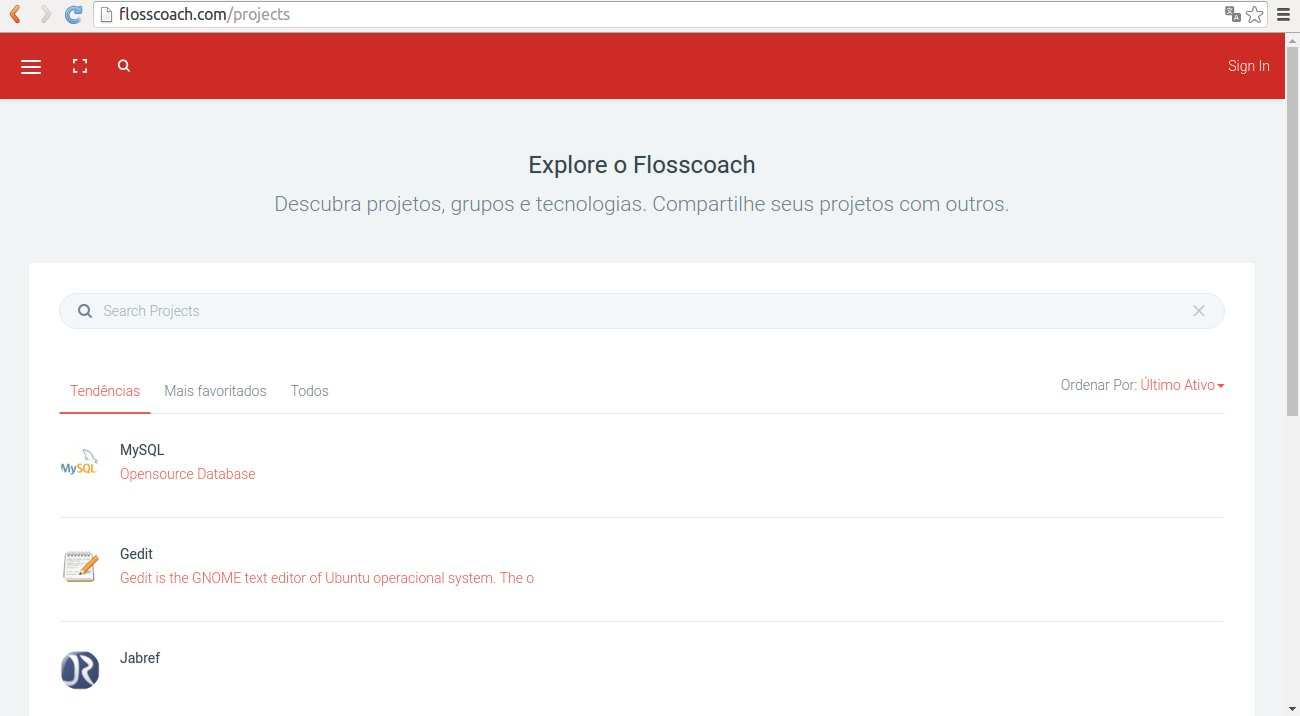
\includegraphics[keepaspectratio=true,scale=0.3]{figuras/flosscoachProducao.eps}
	\caption{Página de projetos do novo portal FlossCoach.}
\end{figure}

\begin{figure}[h]
	\centering
	\label{fig:producao}
		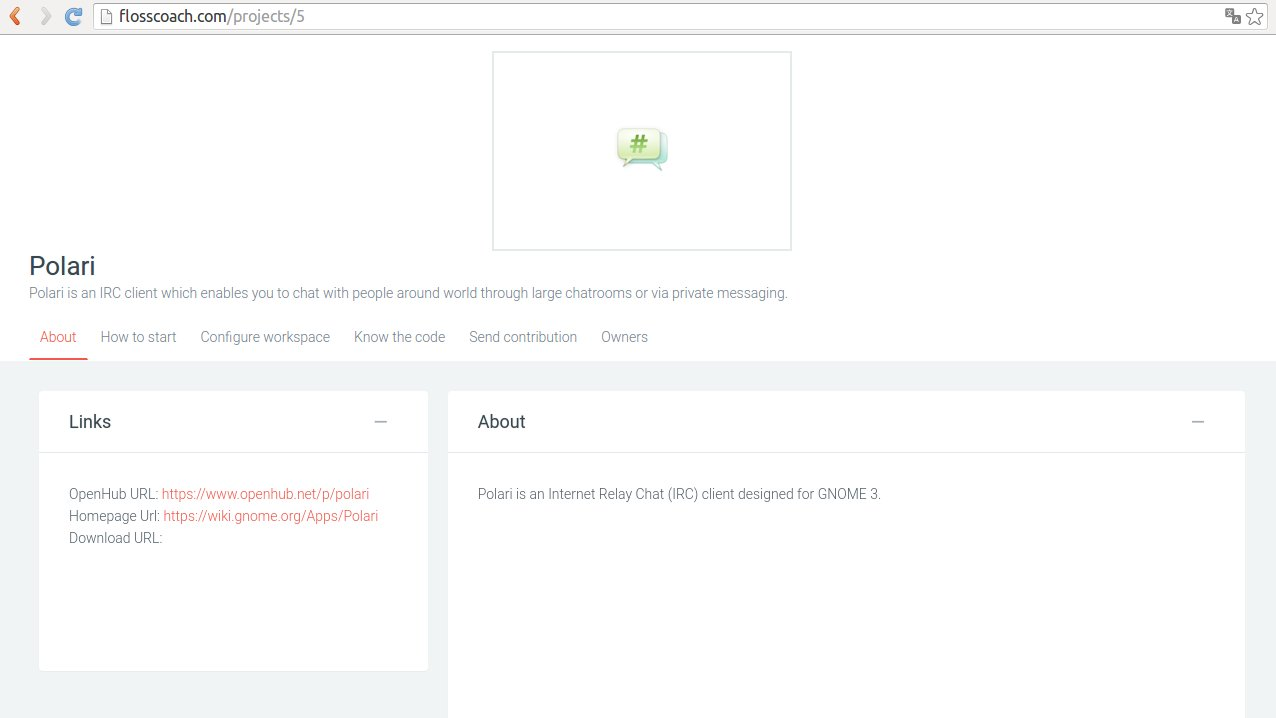
\includegraphics[keepaspectratio=true,scale=0.3]{figuras/paginaprojeto.eps}
	\caption{Página do projeto Polari no novo portal FlossCoach.}
\end{figure}

Passada a \textit{sprint} 4, na disciplina de Manutenção e Evolução de Software é feita uma prática
para verificar quão limpo é o código em que os alunos estão trabalhando utilizando
ferramentas de análise estática onde essas ferramentas apresentam o que pode ser melhorado 
no código para que os software fiquem mais seguros e coesos. Com os destaques feitos pelas
ferramentas a \textbf{Sprint 5} foi separada para fazer a refatoração do código
nos pontos criticados.

Na \textbf{Sprint 6} foram feitas refatorações afim de resolver dívidas técnicas 
que ficaram das \textit{sprints} anteriores. Essas tarefas foram feitas com a intenção 
de deixar as contribuições feitas durante o perído da disciplina completas.  

\begin{figure}[h]
	\centering
	\label{fig:producao}
		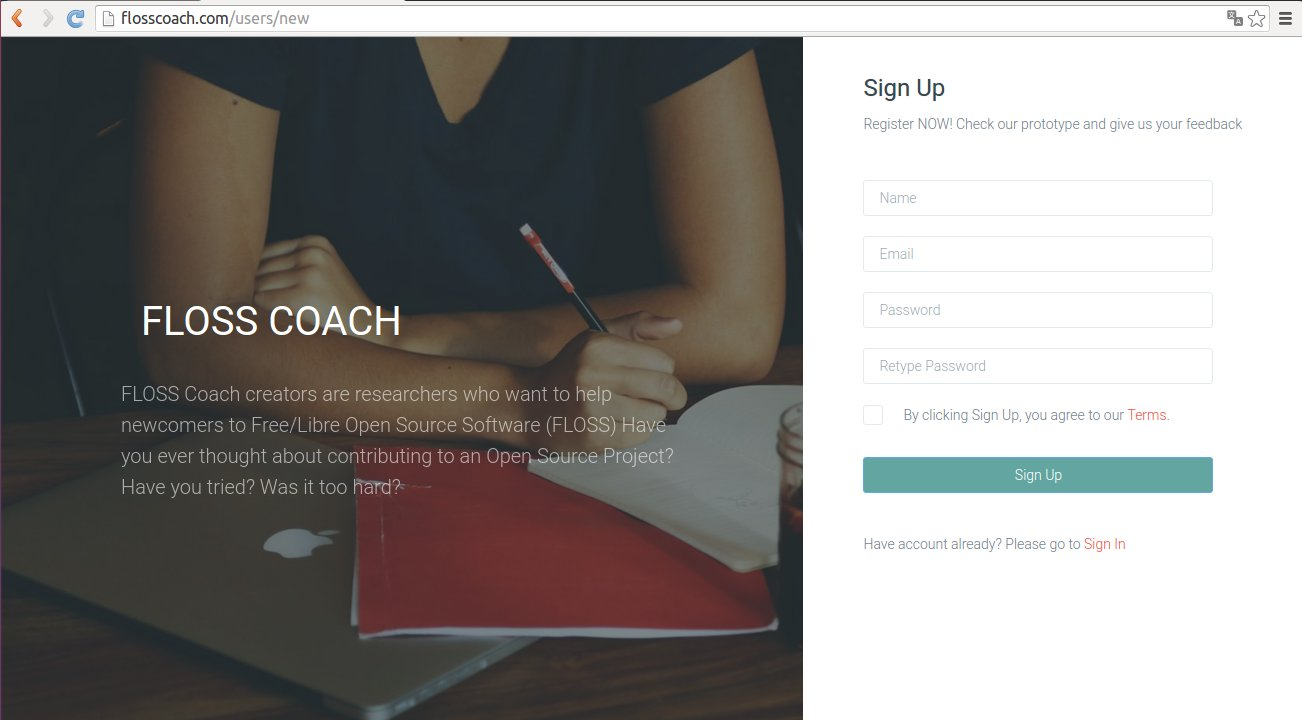
\includegraphics[keepaspectratio=true,scale=0.3]{figuras/cadastrousuario.eps}
	\caption{Página de cadastro de usuário do novo portal FlossCoach.}
\end{figure}

Ao final da terceira fase de desenvolvimento o antigo portal FlossCoach foi substituído pela
nova versão e está disponível na produção no mesmo endereço que estava o antigo, \textit{flosscoach.com}.
Nessa nova versão é possível cadastrar e editar usuário e software, fazer login através das redes sociais 
\textit{Facebook}\footnote{http://facebook.com} e \textit{Twitter}\footnote{http://twitter.com} além do \textit{Github}\footnote{http://github.com}, 
buscar informações a respeito dos projetos no \textit{OpenHub}\footnote{http://openhub.com}. Foi feita a traducão
do portal para português e ele pode ser visto agora tanto em inglês quanto português. Também na nova 
versão do portal já é possível resgatar senha de usuário.

